\documentclass[11pt]{article}
\usepackage{graphicx}
\usepackage{amsmath}
\usepackage{amssymb}
\usepackage{url}
\usepackage{hyperref}
\usepackage{times}
\usepackage{geometry}
\geometry{margin=1in}

\title{Frequency-Domain Logic Encoding for Protocol-Enforced Systems}
\author{Christopher Hirschauer \\ \texttt{c.hirschauer@outlook.com}}
\date{August 30, 2025}

\begin{document}
\maketitle

\begin{abstract}
This paper proposes a novel control architecture that replaces traditional binary logic with
frequency-domain encoding to achieve enhanced semantic density, forensic traceability, and
protocol-level enforcement. By mapping logical states to discrete frequency bands, the system
enables multi-valued logic, intent encoding, and resilient plugin validation. The tradeoff between
raw execution speed and semantic throughput is quantified, and implementation pathways are
outlined for both software simulation and hardware integration.
\end{abstract}

\noindent
\textbf{Keywords:} Protocol-Based Computing, Frequency Encoding, Semantic Logic, Control Architecture, Signal Enforcement

\section{Introduction}
Traditional computing systems rely on binary logic—voltage levels representing 0 and 1—to encode
and execute instructions. While efficient, this model lacks semantic expressiveness and is vulnerable
to default behaviors, abstraction leakage, and audit failure. This paper introduces a frequency-
based logic model where each logical state is represented by a distinct frequency, enabling multi-bit
encoding per signal pulse and enforcing control protocols at the signal layer.

\section{Frequency-Based Logic Model}

\subsection{Encoding Scheme}
\begin{itemize}
  \item Binary Model: 2 frequencies $\rightarrow$ 1 bit per pulse
  \item Hex Model: 16 frequencies $\rightarrow$ 4 bits per pulse
  \item Extended Model: $2^n$ frequencies $\rightarrow$ $n$ bits per pulse
\end{itemize}

Each frequency $f_i$ maps to a semantic intent:
\begin{itemize}
  \item $f_1 = 1 \,\text{kHz}$ — Audit-only
  \item $f_{10} = 10 \,\text{kHz}$ — Override Approved
  \item $f_{16} = 16 \,\text{kHz}$ — Force Rollback
\end{itemize}

\subsection{Control Enforcement}
Execution is gated by frequency validation. Instructions are only executed if the correct frequency
signature is present, ensuring explicit approval and forensic traceability.

\section{Semantic Throughput vs Raw Speed}

\subsection{Semantic Gain}
Hex-frequency encoding delivers 4x semantic payload per signal compared to binary. Reduces signal
count per instruction by 50\%.

\subsection{Speed Tradeoff}
Signal discrimination latency: 30–50\% overhead. Synchronization and filtering introduce MHz-
scale bottlenecks. Net result: slower execution, but higher control fidelity.

\section{Implementation Pathways}

\subsection{Software Simulation}
Frequency-encoded signals can be generated with simple scripts, but time-domain plots of long signals
often compress into unreadable blocks. Instead, frequency-domain visualizations (spectrograms) and
zoomed segments reveal the structure of the encoding.

\begin{figure}[t]
  \centering
  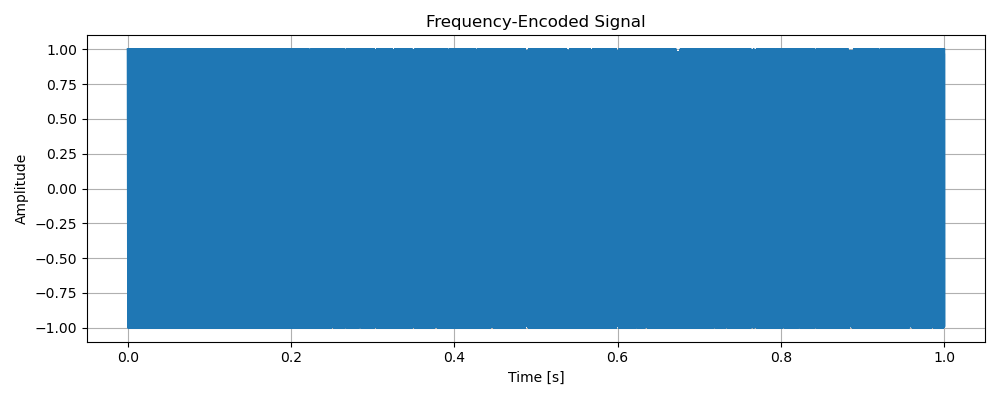
\includegraphics[width=\linewidth]{frequency_encoded_signal.png}
  \caption{Spectrogram of a frequency-encoded control signal sweeping 1–16 kHz across 1 s. Time–frequency view prevents the filled-rectangle artifact of dense time-domain plotting.}
  \label{fig:chirp-spectrogram}
\end{figure}

\begin{figure}[t]
  \centering
  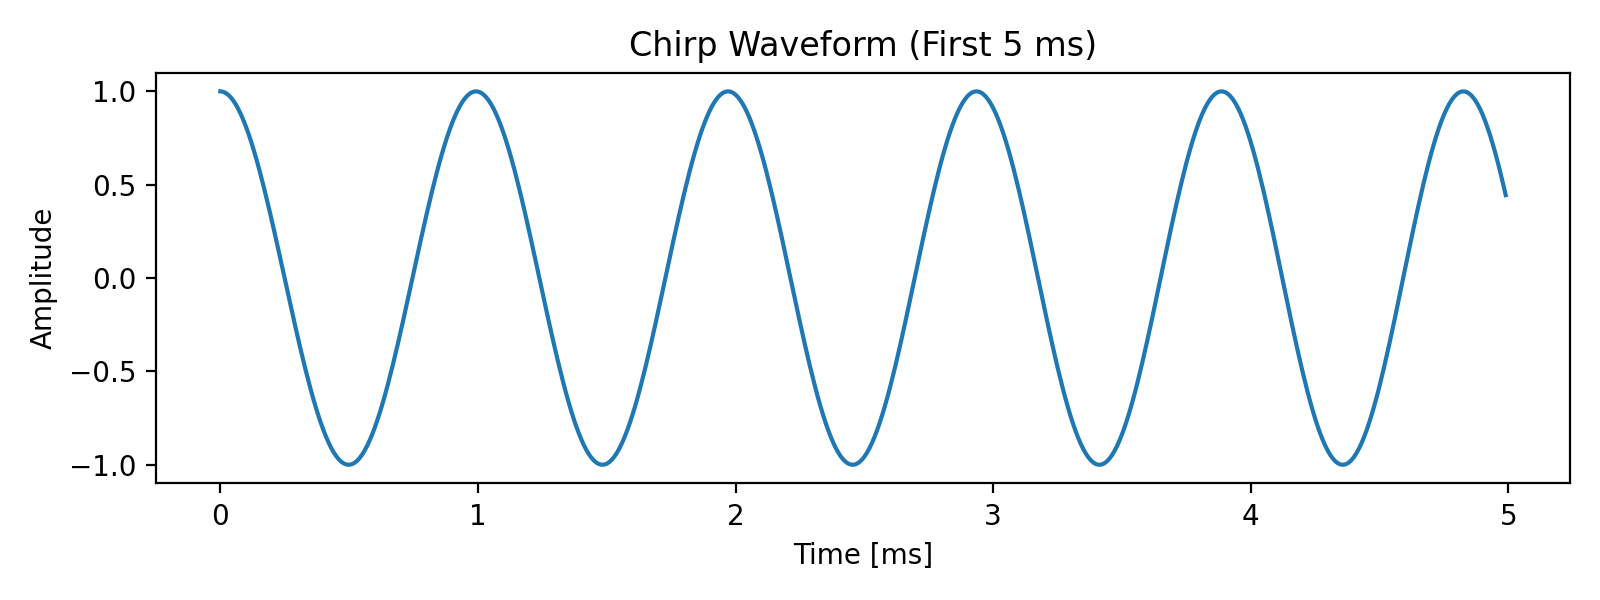
\includegraphics[width=\linewidth]{waveform_zoom.png}
  \caption{Zoomed time-domain view (first 5 ms) of the same signal. Zooming avoids alias-like fill effects and makes oscillations visible.}
  \label{fig:chirp-zoom}
\end{figure}

\begin{figure}[t]
  \centering
  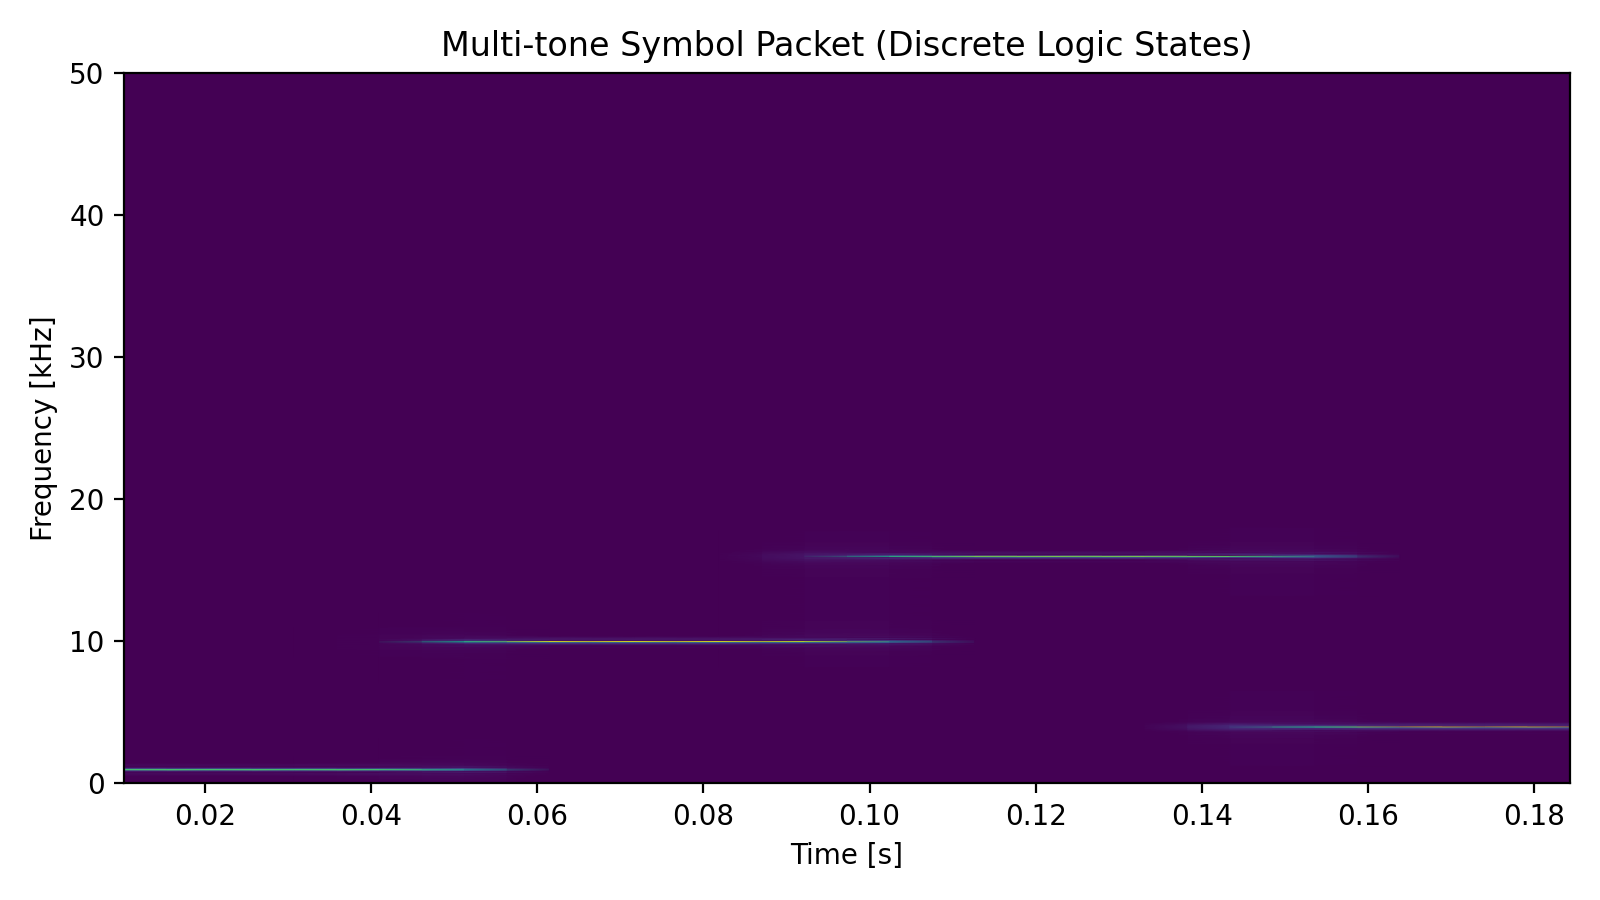
\includegraphics[width=\linewidth]{multitone_packet.png}
  \caption{Multi-tone symbol packet: four discrete states mapped to distinct frequencies (e.g., 1 kHz = \emph{Audit}, 10 kHz = \emph{Override}, 16 kHz = \emph{Rollback}, 4 kHz = \emph{Reserve}). This directly visualizes frequency-as-logic.}
  \label{fig:multitone-packet}
\end{figure}

\subsection{Hardware Integration}
\begin{itemize}
  \item FPGA or DSP-based frequency discriminators
  \item Oscillator banks for signal generation
  \item Analog-to-digital converters for real-time validation
\end{itemize}

\section{Error Modeling and Resilience}
Frequency misclassification can be modeled via Gaussian noise and band overlap. Error correction via
Hamming codes or CRC tagging improves reliability. Redundant fallback frequencies provide recovery
modes.

\section{Applications}
\begin{itemize}
  \item Plugin Recovery Protocols: Frequency-tagged rollback and override signals
  \item AI Instruction Enforcement: GPT directives encoded in waveform pulses
  \item Forensic Logging Systems: Signal-level audit trails with semantic tagging
\end{itemize}

\section{Conclusion}
Frequency-domain logic encoding offers a transformative approach to control architecture, enabling
multi-valued logic, semantic compression, and protocol-level enforcement. While it introduces la-
tency, the tradeoff is justified in systems demanding resilience, auditability, and override protection.
This model redefines the relationship between signal and intent, paving the way for next-generation
protocol-driven computing.

\bibliographystyle{plain}
\bibliography{references,protocol_computing_references}

\end{document}

